\chapter{Metodologia}
\section{Comitê de Ética e Pesquisa}
A coleta de dados foi autorizada pelo Comitê de Ética e Pesquisa da Faculdade da Saúde da UnB CAAE 38386714.8.0000.0030 e foi realizado pelos pesquisadores Jorge Luiz (Engenheiro Eletricista) e Bruna da Silva (Fisioterapeuta).

Ela utiliza o protocolo descrito no Anexo \ref{apendicprotocolo}, o qual descreve detalhadamente todo o processo de coleta dos dados, bem como o Termo de Consentimento Livre e Esclarecido – TCLE encontra-se no Anexo \ref{apendicetae}.

\section{Processo de construção de uma aplicação de Aprendizado de Máquina}

Segundo \citeonline{Amazon} e \citeonline{geron2017hands}, o processo de desenvolvimento de uma aplicação de AM é iterativo e envolve uma série sequencial de passos, que de maneira geral vão desde entender o quadro geral até a apresentação da solução da proposta da aplicação. O processo pode ser visualizado pela representação BPMN (sigla do inglês: \textit{Business Process Model and Notation}, Modelo e Notação de Processos de Negócio) na Figura \ref{ProcessoAM}.

\begin{figure}[h]
	\centering
	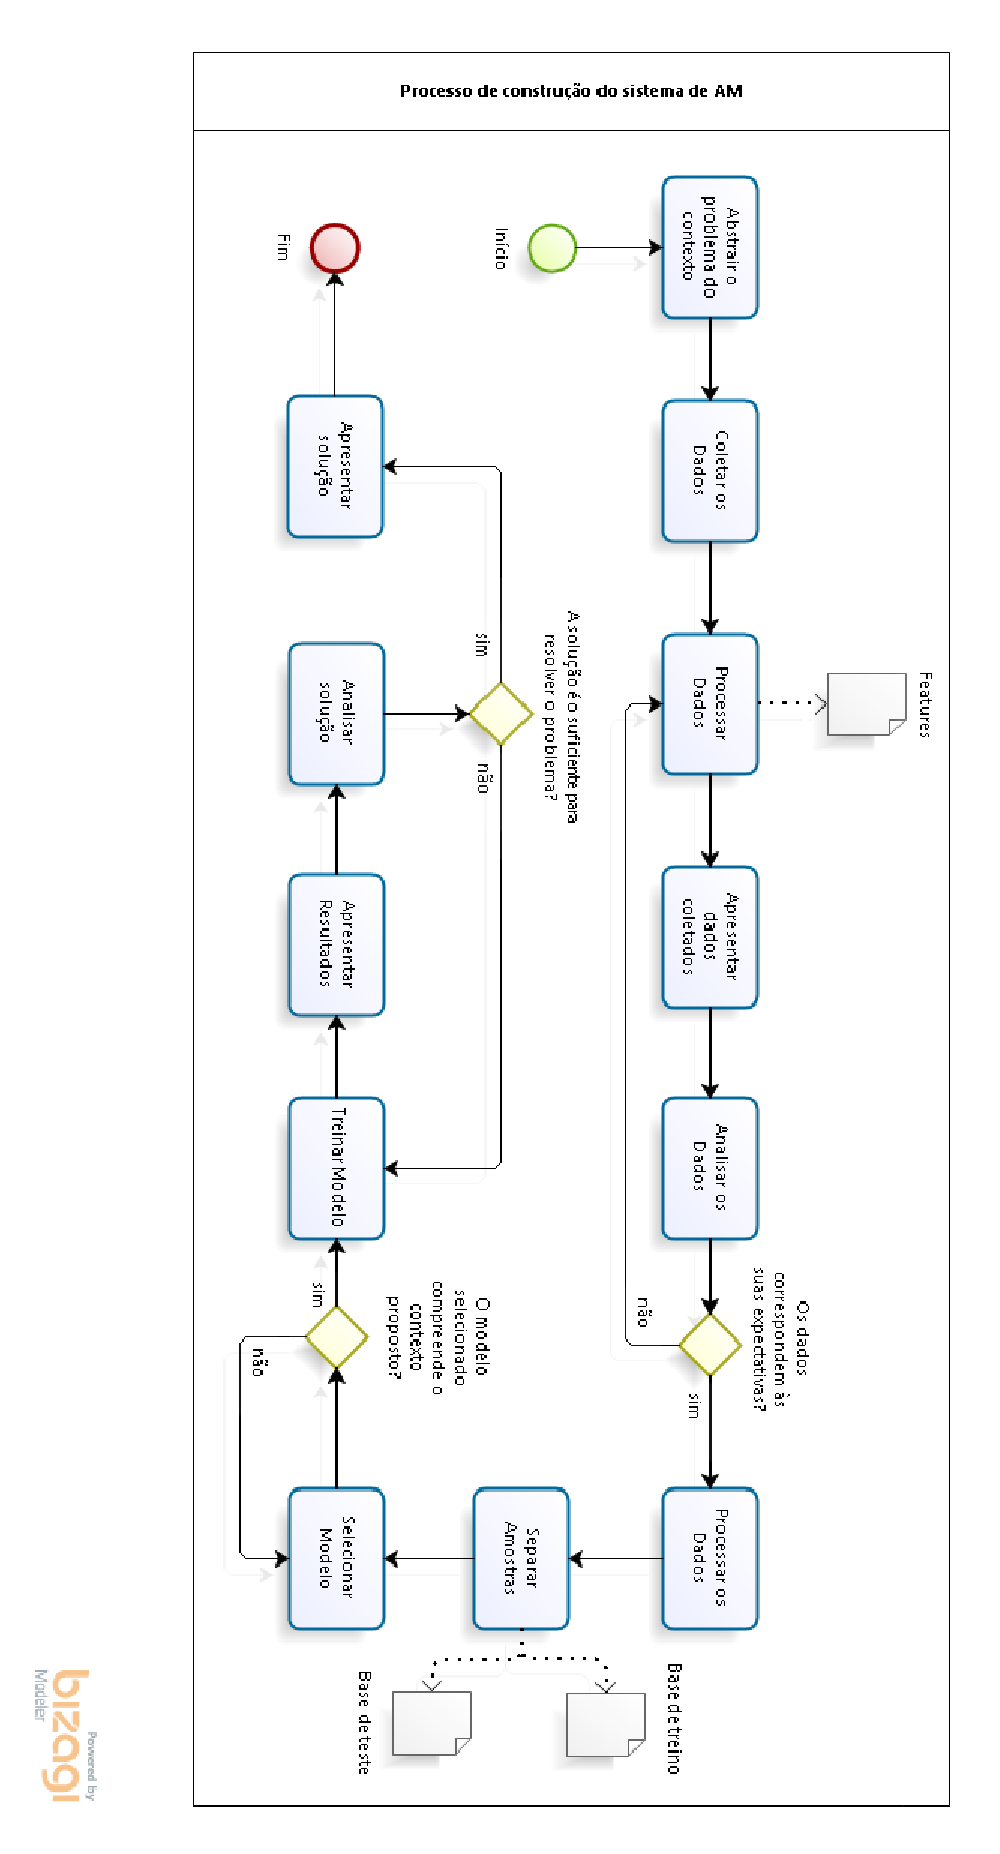
\includegraphics[width=1\textwidth]{figuras/ProcessoAM.eps}
	\caption{Diagrama do processo (Imagem do autor).}
	\label{ProcessoAM}
\end{figure}

\subsection{Abstrair o problema no contexto}
O primeiro passo é entender o que será predito, ou seja, analisar a natureza do problema observando quais respostas o modelo escolhido deverá predizer, para auxiliar na solução do problema \cite{geron2017hands}.

Tendo em vista o seguinte cenário, no qual é necessária a fabricação de produtos, porém a decisão de qual produto fabricar depende do número de vendas em potencial. Nesse cenário, é necessário saber a quantidade de vezes que cada produto foi comprado, ou seja, predizer o número de vendas. Existem diversas maneiras de definir esse problema utilizando AM, porém a escolha de como definir o problema depende do caso de uso ou necessidade comercial \cite{Amazon}.

Um ponto importante do entendimento do contexto é a abstração do problema. Essa etapa tem um papel fundamental na escolha dos modelos, pois tendo se entendido a natureza do problema, será selecionado o modelo para predizer os resultados com base no tipo de aprendizado mais adequado a este contexto. Além disso, é necessário definir claramente quais os objetivos deverão ser atingidos, qual a métrica de desempenho utilizar para validar o modelo e quais algoritmos utilizar para alcançar o desempenho esperado. Com estas e outras respostas será possível enquadrar o problema em supervisionado, não supervisionado ou por reforço e após isso categoriza-lo em classificação, regressão \cite{geron2017hands}. Essa etapa de análise tem como finalidade orientar o trabalho evitando a criação de modelos que não respondem o problema, além de otimizar o esforço no desenvolvimento \cite{Amazon}.

\subsection{Coleta de dados}

Os dados coletados nessa etapa devem estar ligados diretamente ao que é requerido pelo problema. Atender esses requisitos a fim de atender as necessidades do contexto é de suma importância, pois alguns dos já citados desafios encontrados no desenvolvimento de sistema de AM estão relacionados aos dados que serão utilizados \cite{geron2017hands}.

A quantidade de dados coletados nessa etapa ainda é incerta, porém é levado em consideração que quanto maior a quantidade de dados coletados, melhor. Neste trabalho são utilizados sinais captados por dispositivos sEMG, mais informações sobre esse sinal são apresentadas na seção \ref{ch:sEMG}.

\subsection{Analisar os Dados}

Antes de passar os dados para o algoritmo de AM, é considerado uma boa prática inspecionar seus dados para identificar problemas e obter \textit{insights} sobre os dados que se está utilizando \cite{Amazon}, quanto melhor forem os dados, melhor será o modelo preditivo que está utilizando esses dados.

Segundo \citeonline{Amazon}, enquanto você está analisando seus dados é importante responder às seguintes perguntas:
\begin{itemize}
	\item Os dados correspondem às suas expectativas?
	\item Houveram problemas nas coletas dos dados?
	\item Quais classes são as mais frequentes dentre os seus dados?
	\item Existem mais valores ausentes ou inválidos do que o esperado?
\end{itemize}

Além de construir um resumo dos dados relacionados a essas perguntas, também é uma boa prática conhecer a correlação entre cada variável e a classe de destino. Em geral, é necessário incluir variáveis com alta correlação, porque elas possuem maior poder preditivo (sinal) e deixam de fora as variáveis com baixa correlação, porque são provavelmente irrelevantes \cite{Amazon}.

Essas práticas são importantes para conhecer os dados que serão utilizados podendo prevenir ou facilitar a identificação de possíveis erros futuros com relação a utilização dos dados.

\subsection{Processar Dados}

Após a etapa de análise dos dados, é necessário tornar as variáveis mais significativas. Esta etapa é conhecida como processamento de \textit{features}, sendo responsável por preparar os dados para serem consumidos pelos algoritmos de AM e pode ser resumida em três etapas mais comuns \cite{blum1997selection}:

\begin{enumerate}
	\item \textbf{Formatar}: Os dados selecionados podem não estar no formato desejado ou os dados estão em um banco de dados relacional e é desejado que os mesmos estejam em um arquivo simples. Formatar os dados para um padrão que facilita o trabalho com esses dados é a primeira etapa do processamento.
	\item \textbf{Limpar}: Remover ou consertar os dados que faltam dentro de um banco de dados  Pode haver instâncias de dados incompletas e não conter os dados para solucionar o problema. Essas instâncias podem precisar ser removidas. Além disso, pode haver informações confidenciais em alguns dos atributos e esses atributos podem precisar ser anonimizados ou removidos dos dados completamente.
	\item \textbf{Selecionar Amostras}: No caso de se trabalhar com uma grande massa de dados, nem sempre todos esses dados serão utilizados. A quantidade exagerada de dados pode levar à tempos de execução muito elevados e maiores requisitos computacionais. Selecionar uma amostra representativa dos dados selecionados pode ser muito mais rápida para explorar os resultados.
\end{enumerate}

\subsection{Selecionar o Modelo}
Após identificar o problema, explorar os dados, limpar as incoerências e separar os dados em treino e teste, é possível escolher o modelo adequado para solucionar o problema identificado \cite{geron2017hands}.

\subsection{Treinar o Modelo}
Para treinar o modelo, com a totalidade do dados separados em, por exemplo, 70\% dados de treino e 30\% em dados de teste. Utiliza-se os 70\% dos dados para treinar o modelo, passando estes dados pelo algoritmo escolhido, e os outros 30\% restantes serão utilizados para testar a eficiência do modelo.

\subsection{Validar a solução}
Para validar a solução, utiliza-se a validação cruzada, a qual foi descrita na seção \ref{sc:crossvalidation}. Também é comum a utilização da matriz de confusão descrita na seção \ref{sc:matrizconsusao}.

\subsection{Apresentar a solução}
A tecnologia utilizada para o desenvolvimento neste trabalho, \textit{Python}, possui muitas bibliotecas complementares para fazer visualizações estáticas ou dinâmicas, mas focaremos principalmente na combinação entre \textit{Matplotlib}, \textit{Numpy} e \textit{Pandas}.
